\section{Analisi dei requisiti}
La presente sezione ha lo scopo di analizzare i servizi che il sito web finale deve offrire agli utenti e quali caratteristiche funzionali e qualitative devono essere garantite.

\subsection{Interazione degli utenti}
%cosa gli utenti possono fare? Quali attività/servizi offriamo?
[descrivi]

\begin{figure}[H]
	\centering
	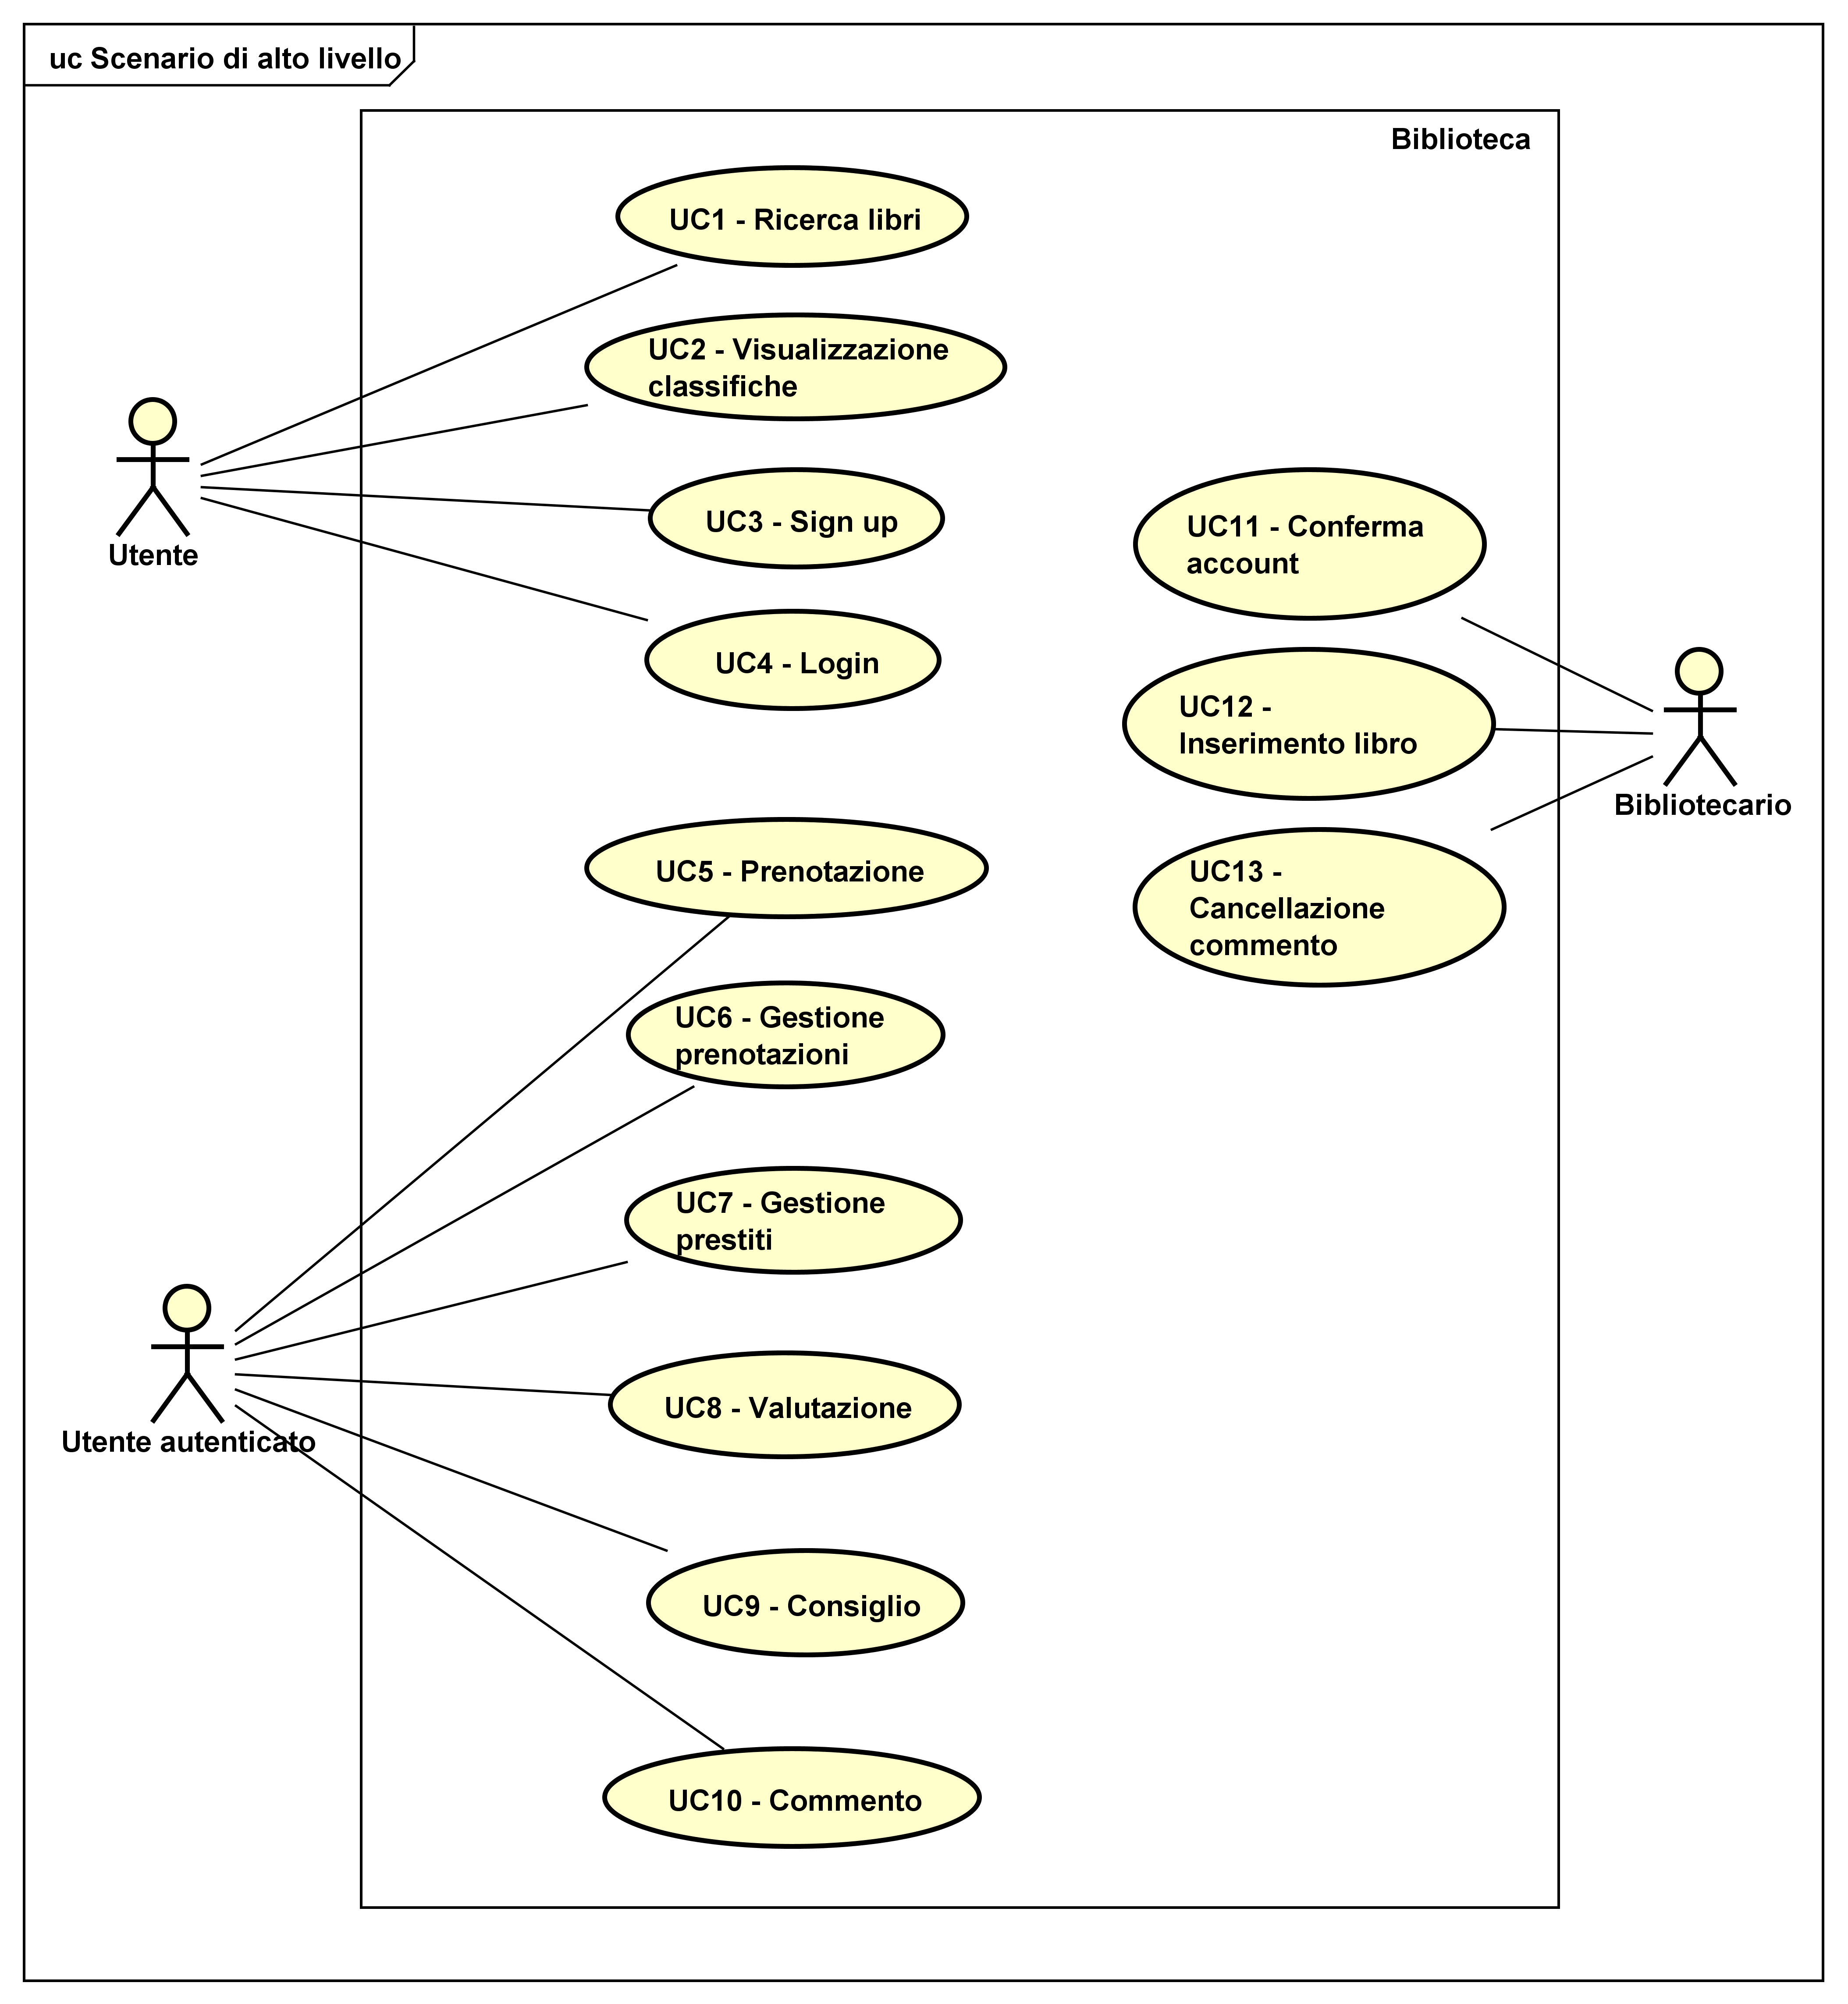
\includegraphics[width= 14cm]{immagini/user_case.png}
	\caption{Visione di alto livello dei principali casi d'uso}
\end{figure}


\subsection{Aggiornamenti e amministrazione}
%definisci il progesso di aggiornamento del sito.. Come si aggiungono contenuti? Ogni quanto?


\subsection{Organizzazione e mappa del sito}
%che struttura ha il sito?

\subsection{Performance}
%quali sono gli indicatori e cosa ci si aspetta


\subsection{Accessibilità}


\subsection{Sicurezza}